
%(BEGIN_QUESTION)
% Copyright 2007, Tony R. Kuphaldt, released under the Creative Commons Attribution License (v 1.0)
% This means you may do almost anything with this work of mine, so long as you give me proper credit

The following loop diagram documents a wastewater pH neutralization system, adding acid or caustic as needed to the water to maintain a relatively neutral pH level:

$$\includegraphics[width=15.5cm]{i02002x01.eps}$$

Determine the following parameters within this system, assuming a controller output of 64\%, a measured pH of 7.5, and negligible wire resistance:

\begin{itemize}
\item{} Voltage between terminals 22 and 21 on the controller = \underbar{\hskip 50pt} V
\vskip 10pt
\item{} Voltage between terminals 3 and 4 of terminal block TB-2 = \underbar{\hskip 50pt} V
\vskip 10pt
\item{} Which control valve is completely shut: the {\it caustic valve} or the {\it acid valve} ?
\vskip 10pt
\item{} Position of open valve = \underbar{\hskip 50pt} \% open 
\vskip 10pt
\item{} Direction that integral control action will drive the controller output, assuming a setpoint of 8 pH: {\it increase} or {\it decrease}?
\end{itemize}

\underbar{file i02002}
%(END_QUESTION)





%(BEGIN_ANSWER)

\begin{itemize}
\item{} Voltage between terminals 22 and 21 on the controller = \underbar{\bf 3.143} V
\vskip 10pt
\item{} Voltage between terminals 3 and 4 of terminal block TB-2 = \underbar{\bf 5.012} V
\vskip 10pt
\item{} Which control valve is completely shut: the {\bf acid valve}
\vskip 10pt
\item{} Position of open valve = \underbar{\bf 28}\% open 
\vskip 10pt
\item{} Direction that integral control action will drive the controller output, assuming a setpoint of 8 pH: {\bf increase} (adding more caustic to the water)
\end{itemize}

%(END_ANSWER)





%(BEGIN_NOTES)

{\bf This question is intended for exams only and not worksheets!}.

%(END_NOTES)


